\chapter{Introduction\label{chap:introduction}}

With many Earth-like features such as obliquity seasons (“summer” and “winter”), polar ice caps, a similar rotation period, and evidence suggesting that liquid water once existed on its surface\cite{clancyetalChapter022017}, Mars is an intriguing subject of study, which can help us understand how physical processes interact to shape a planet’s climate and drive its changes\cite{Leovy1978}. A key factor driving climatic processes on Mars is wind and atmospheric circulation. It has not only shaped Mars' surface over time but plays a crucial role in the transport of water vapor, dust, trace gases, and heat. Although understanding wind patterns is highly relevant for future human exploration, they are still considered a major unknown\cite{Guzewich2021}.

\section{Historical Background}

The earliest efforts to determine wind flows on Mars, published in 1950 by Seymour Hess, were based on pixelated photographs taken during the planet's northern hemisphere winter, yielding 18 wind vectors as shown in Figure 1.1\cite{Seymour1950}. 
\FloatBarrier
\begin{figure}[h!] 
    \centering
    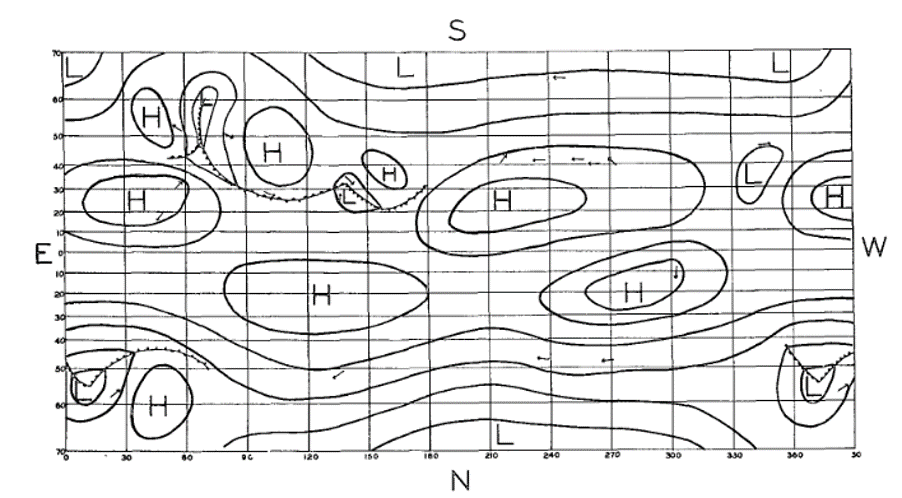
\includegraphics[width=1\textwidth]{fig_01.png}
    \caption{A schematic streamline map for Mars in northern hemisphere winter by Seymour Hess, where arrows represent observed cloud drift directions\cite{Seymour1950}. }
\end{figure}
\FloatBarrier
However, as technology progressed, instrumental capabilities gradually improved. The launch of the Hubble Space Telescope in 1990 provided high-resolution ultraviolet and visible light images taken above the distorting effects of the Earth’s atmosphere\cite{Uri2020}, enabling a detailed, pixel-based longitude-wise analysis of the Martian aphelion cloud belt\cite{Wolff1999}. The successful landing of Pathfinder in 1997 marked the introduction of on-surface measurements, as it recorded atmospheric data during its descent and conducted meteorological measurements at the landing site\cite{NasaMarsPathfinder}. While on-surface measurements from Pathfinder and subsequent missions like the Mars Exploration Rover and Phoenix Mars Lander offer excellent local coverage, orbital observations, which began with the Mars Global Surveyor in 1988 and continued with missions such as NASA's Mars Odyssey and Mars Reconnaissance Orbiter\cite{clancyetalChapter022017}, provide global coverage that facilitates the analysis of wind patterns on a larger scale.

\section{Cloud Tracking}

While the idea of tracking clouds using planetary-type imagery has been around since Robert Hooke observed a moving spot in one of the belts of Jupiter in the 16th century\cite{Hooke1665}, non-manual tracking of atmospheric motion was properly established as a practice in the 1960s, shortly after the first meteorological satellites were launched\cite{Menzel2001}. Since then, various tracking methods have evolved and been applied across diverse fields of research requiring motion tracking. Among these, optical flow and cross-correlation algorithms have emerged as techniques delivering efficient results not only in studies of e.g. fluid mechanics but also in large-scale cloud tracking in planetary atmospheres. 



